\chapter{Relativité restreinte : référentiels, simultanéité et transformation de Lorentz}

La relativité est le principe selon lequel les lois de la physique ne dépendent pas du référentiel inertiel choisi pour les décrire. Notre première tâche relève de la cinématique : il s’agit de comprendre l’espace, le temps, le mouvement, la synchronisation et la transformation qui fait passer d’un référentiel inertiel à un autre. Nous étudierons ensuite la dynamique, avec l’énergie relativiste, la quantité de mouvement, la force, l’analogue de l’équation du mouvement de Newton et le sens de \(E=mc^2\). Une fois ces bases établies, nous pourrons aborder la relativité générale sous un angle conceptuel, à travers l’espace-temps courbe, le mouvement de particules dans un champ gravitationnel donné, les trous noirs et l’expansion de l’Univers, sans commencer par le difficile problème de la résolution des équations de champ d’Einstein.

Il convient de distinguer la rigueur conceptuelle de la rigueur mathématique. Nous n’utiliserons pas d’approximation dont nous savons qu’elle est fausse. Nous mettrons plutôt l’accent sur les effets d’un champ gravitationnel sur les horloges, les particules et la géométrie, tout en reportant l’étude des outils nécessaires à la construction de solutions arbitraires des équations de champ. La relativité restreinte doit être traitée plus explicitement, car toute la réflexion qui suit repose sur sa cinématique.

Il faut donc commencer non par une formule célèbre, mais par une description précise de ce qu’un observateur entend par lieu et par instant.

\section{Un référentiel est un système de coordonnées physique}

Imaginons l’espace rempli d’un réseau arbitrairement fin de règles graduées en mètres. Chaque nœud du réseau est repéré par trois coordonnées spatiales et porte une horloge. Ensemble, les règles et les horloges constituent un référentiel.

\begin{definition}Un \emph{événement} est quelque chose qui se produit en un lieu et à un instant. Dans une dimension spatiale, ses coordonnées s’écrivent \((x,t)\) ; dans trois dimensions, elles s’écrivent \((x,y,z,t)\).\end{definition}

La physique newtonienne ajoute une hypothèse forte : toutes les horloges idéales peuvent être synchronisées une fois pour toutes. Le temps est universel. On peut déplacer une horloge, ou un observateur peut porter une montre, mais tout le monde est censé s’accorder sur le même \(t\) partout. On parle parfois de temps absolu ; on peut se le représenter comme le temps de Dieu, une horloge unique pour le monde entier.

Le principe de relativité est antérieur à Einstein. On peut se le représenter par un train roulant à vitesse parfaitement uniforme sur des rails si lisses que rien ne cahote ni ne tremble. À l’intérieur, on peut lancer et rattraper des balles exactement comme dans un train à l’arrêt en gare. Jongler constitue une expérience de mécanique étonnamment complète : elle exige de mesurer le temps, de tenir compte de la gravité, de viser juste et de contrôler à plusieurs reprises les trajectoires. Si le train se déplace à vitesse constante, aucune de ces règles ne change. Une balle lancée verticalement retombe dans la même main ; le train ne se dérobe pas sous elle. Galilée a reconnu ce fait, et Newton l’a formulé systématiquement dans ses lois du mouvement.

Avant Galilée, on pouvait être tenté de penser que le train en mouvement avançait pendant que la balle était en l’air, obligeant le jongleur à tendre le bras vers l’arrière ou vers l’avant pour la rattraper. L’erreur consiste à oublier que la balle possède déjà la vitesse horizontale du train au moment où elle quitte la main. Aucune expérience réalisée à bord du wagon qui roule sans à-coups ne révèle un état privilégié de repos absolu. Seul le mouvement relatif entre les deux trains est observable.

Le train immobile et le train en mouvement uniforme constituent donc deux référentiels inertiels. Avant Einstein, ils étaient reliés par des transformations galiléennes.

\section{Représenter l’espace-temps}

Pour l’instant, nous laissons de côté \(y\) et \(z\) et représentons le temps verticalement et la position \(x\) horizontalement. Chaque point du dessin correspond à un événement. La droite \(x=0\) représente l’histoire, ou la \emph{ligne d’univers}, de l’origine spatiale. Les droites verticales voisines \(x=1,2,3,\ldots\) représentent les lignes d’univers des autres nœuds du réseau. Les droites horizontales regroupent les événements qui ont un même instant.

\begin{figure}[H]\centering
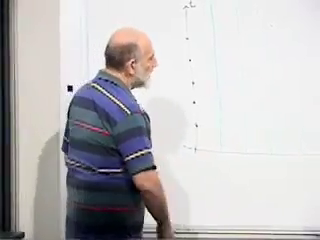
\includegraphics[width=0.62\textwidth]{lecture_01_figure_02.png}\caption{L’axe du temps dans le référentiel au repos et les premières lignes d’univers du réseau spatial.}\lectureframe{00:16:38}\end{figure}

On voit mieux cette même construction dans un schéma idéalisé :

\begin{figure}[H]\centering
\begin{tikzpicture}[scale=0.95]
\draw[->] (-1.2,0) -- (5.2,0) node[right] {$x$};
\draw[->] (0,-0.2) -- (0,4.8) node[above] {$t$};
\foreach \x in {-1,1,2,3,4}
  \draw[gray!65] (\x,0) -- (\x,4.4);
\foreach \y in {1,2,3,4}
  \draw[gray!65] (-1.0,\y) -- (4.4,\y);
\fill (0,0) circle (1.5pt);
\node[below left] at (0,0) {$0$};
\node[left] at (0,1) {$1$};
\node[left] at (0,2) {$2$};
\node[left] at (0,3) {$3$};
\node[below] at (1,0) {$1$};
\node[below] at (2,0) {$2$};
\node[below] at (3,0) {$3$};
\end{tikzpicture}\caption{Un réseau d’espace-temps au repos. Les droites verticales correspondent à une position constante ; les droites horizontales, à un instant constant.}\end{figure}

Le réseau est imaginaire et son espacement est arbitraire. On peut utiliser des mètres, des centimètres, des microns ou tout intervalle encore plus petit qui ait un sens physique. Il sert à attribuer des coordonnées précises à chaque événement.

L’expression « référentiel » prend maintenant un sens opérationnel. Elle ne désigne pas simplement un point de vue ou une personne qui regarde dans une direction donnée. C’est un dispositif de coordonnées étendu. Pour un événement donné, les règles locales indiquent où il s’est produit et l’horloge locale, quand. On peut alors comparer d’autres grandeurs physiques entre référentiels : la position et la vitesse d’une particule, son énergie, éventuellement la température d’un corps et, par la suite, sa quantité de mouvement et la force. La comparaison la plus simple porte sur \(x\) et \(t\) ; c’est par là que nous commencerons.

Plaçons maintenant un second réseau sur un train qui se déplace dans la direction positive de \(x\) à vitesse constante \(v\). Faisons coïncider les origines à \(t=0\). L’origine mobile suit alors la trajectoire
\begin{equation}
x=vt.
\end{equation}
Tout autre point fixe dans le train suit une ligne d’univers inclinée parallèle. Cette inclinaison exprime simplement le fait que le train change de position au fil du temps.

Supposons que le point arrière du train soit l’origine primée. À \(t=0\), elle coïncide avec l’origine de la gare. À un instant ultérieur \(t\), sa coordonnée dans le référentiel de la gare est \(vt\). Un événement voisin de coordonnée \(x\) ne se trouve donc qu’à une distance \(x-vt\) de l’origine du train. C’est pourquoi la transformation fait intervenir une soustraction, et non une règle algébrique arbitraire.

Notons \((x,t)\) les coordonnées d’un événement dans le référentiel de la gare et \((x',t')\) celles du même événement dans le référentiel du train. Pour Galilée et Newton, le temps reste universel :
\begin{equation}
t'=t.
\end{equation}
Pendant le temps \(t\), l’origine mobile avance de \(vt\) ; la distance entre cette origine et l’événement vaut donc
\begin{equation}
x'=x-vt.
\end{equation}
En réunissant ces relations,
\begin{align}
t'&=t, & x'&=x-vt.
\label{eq:galilean-forward}
\end{align}
On obtient la transformation inverse en isolant les coordonnées non primées :
\begin{align}
t&=t', & x&=x'+vt'.
\label{eq:galilean-inverse}
\end{align}

\begin{figure}[H]\centering
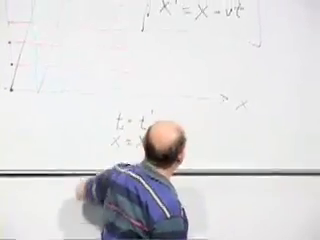
\includegraphics[width=0.72\textwidth]{lecture_01_figure_03.png}\caption{La transformation galiléenne, écrite à côté des deux réseaux d’espace-temps.}\lectureframe{00:21:57}\end{figure}

Le premier couple d’équations indique à l’observateur mobile comment convertir les coordonnées données par l’observateur au repos. Le couple inverse effectue la conversion en sens contraire. Cette conversion réciproque entre descriptions constitue le contenu mathématique de la relativité galiléenne.

Dans la formule spatiale inverse, la substitution \(t\to t'\) ne pose pas de problème uniquement parce que la théorie galiléenne a déjà posé \(t=t'\). Il est utile de relever cette hypothèse dès maintenant. Dans la théorie d’Einstein, les deux coordonnées temporelles différeront, et de telles substitutions ne seront plus automatiques.

\begin{classroomqa}\audiencequestion{Si l’on emporte une horloge puis qu’on la ramène, comment savoir que son mouvement ne l’a pas d’abord accélérée puis ralentie, masquant ainsi l’effet lorsqu’on compare les horloges ?\lecturetimestamp{00:23:09}}\lecturerresponse{Galilée n’aurait pas pu établir le caractère universel du temps avec la précision moderne ; il s’agissait d’une hypothèse physique. On peut la mettre à l’épreuve de nombreuses façons : transporter de bonnes horloges dans des directions opposées, refaire le trajet vers le nord--le sud autant que vers l’est--l’ouest, faire tourner une horloge autour de l’autre ou échanger des signaux horaires sans rapprocher les horloges. Aux vitesses ordinaires, tous ces tests concordent avec une très grande précision. Avec des horloges suffisamment précises ou des vitesses assez élevées, un faible écart apparaît. La défaillance du temps universel n’est pas un défaut de l’expérience : c’est un phénomène que la relativité restreinte doit expliquer.}\end{classroomqa}

\section{Invariants galiléens et loi de Newton}

Un invariant est une grandeur sur laquelle s’accordent tous les observateurs inertiels considérés. Les coordonnées elles-mêmes ne sont pas nécessairement invariantes. Il importe de savoir si les lois qu’on formule à partir d’elles conservent la même forme.

Le terme s’emploie comme nom et comme adjectif. Un nombre peut être un invariant, tout comme une équation peut être invariante sous une transformation. Distinguer les grandeurs invariantes des lois invariantes évite une confusion fréquente : la relativité ne prétend pas que tous les observateurs obtiennent les mêmes coordonnées pour tout. Elle affirme que la loi physique qui relie leurs mesures conserve la même forme.

Considérons deux événements simultanés situés aux positions \(x_1\) et \(x_2\). L’équation~\eqref{eq:galilean-forward} donne
\begin{align}
x_1'&=x_1-vt,\\
x_2'&=x_2-vt.
\end{align}
Leur séparation vaut donc
\begin{equation}
x_2'-x_1'=(x_2-vt)-(x_1-vt)=x_2-x_1.
\end{equation}
En physique galiléenne, la distance entre des événements qui se produisent au même instant est invariante, même si leurs positions respectives ne le sont pas.

\begin{classroomqa}\audiencequestion{Les deux occurrences de \(t\) dans cette soustraction représentent-elles vraiment le même instant ?\lecturetimestamp{00:28:16}}\lecturerresponse{Oui. Nous avons délibérément choisi deux événements \((x_1,t)\) et \((x_2,t)\) simultanés. Ils se trouvent sur une même droite horizontale de temps constant. Le terme commun \(vt\) s’annule donc. Si les événements se produisaient à des instants différents, ce raisonnement ne permettrait pas d’établir l’invariance de leur séparation spatiale.}\end{classroomqa}

Décrivons maintenant une particule par une trajectoire \(x(t)\). L’observateur du train lui attribue
\begin{equation}
x'(t)=x(t)-vt.
\end{equation}
En dérivant une fois, on obtient la règle usuelle d’addition des vitesses :
\begin{equation}
\frac{dx'}{dt}=\frac{dx}{dt}-v.
\end{equation}
La position et la vitesse dépendent du référentiel. Un observateur qui accompagne une flèche la voit se déplacer moins vite qu’un observateur placé au bord de la voie.

Dérivons une seconde fois. Comme la vitesse relative \(v\) est constante,
\begin{equation}
\frac{d^2x'}{dt^2}=\frac{d^2x}{dt^2}.
\end{equation}
L’accélération est invariante sous une transformation galiléenne. Cela suggère fortement pourquoi la loi de Newton s’exprime en fonction de l’accélération plutôt que de la position ou de la vitesse.

Il s’agit de l’accélération d’un objet observé, et non de celle de l’observateur dans le train. Les deux référentiels sont inertiels ; aucun n’accélère par rapport à l’autre. Dans chaque description, des objets peuvent accélérer vers la gauche ou vers la droite, et les deux observateurs s’accordent sur la valeur de cette accélération, même s’ils ne s’accordent pas sur la position ni sur la vitesse de l’objet.

Supposons que deux particules exercent l’une sur l’autre une force qui dépend uniquement de leur séparation mesurée au même instant. Cette séparation étant invariante, la force l’est aussi. Si la masse est également une propriété intrinsèque, indépendante du référentiel, chaque observateur inertiel peut écrire
\begin{equation}
F=ma
\end{equation}
exactement sous la même forme. La mécanique newtonienne est invariante sous les transformations galiléennes. Ce n’est pas seulement plausible : dans le domaine des vitesses ordinaires, elle est extraordinairement précise.

Le raisonnement s’applique aux forces centrales usuelles, comme la gravitation newtonienne ou l’électrostatique, dont l’intensité dépend de la distance. Tous les observateurs galiléens s’accordant sur cette distance à un instant donné, ils s’accordent aussi sur la force. Puisque la force et l’accélération sont fixées, la cohérence exige alors qu’ils s’accordent également sur la masse : un objet d’un kilogramme reste un objet d’un kilogramme lorsqu’il passe dans un train. Chaque symbole de \(F=ma\) s’inscrit dans la même structure invariante.

\section{La lumière ne suit pas la règle galiléenne}

L’électromagnétisme pose problème. Les équations de Maxwell prédisent des ondes qui se propagent dans le vide à une vitesse bien déterminée \(c\). Si les équations de Maxwell sont des lois de la nature et que celles-ci sont les mêmes dans chaque référentiel inertiel, alors tous les observateurs inertiels doivent mesurer la même valeur de \(c\).

La cinématique galiléenne prédit autre chose. Dans le référentiel au repos, une impulsion lumineuse qui se déplace vers la droite satisfait
\begin{equation}
x=ct.
\end{equation}
En appliquant la transformation spatiale, on obtient
\begin{equation}
x'=x-vt=(c-v)t.
\end{equation}
Comme \(t'=t\), l’observateur du train mesurerait la vitesse \(c-v\).

La contradiction peut se formuler sans ambiguïté. Si les équations de Maxwell conservent leur forme, elles prédisent \(c\) dans le référentiel primé. Si l’on conserve la transformation galiléenne, celle-ci prédit \(c-v\). Ces deux prédictions ne peuvent être exactes simultanément lorsque \(v\ne0\).

Ce résultat semble tout à fait naturel si la lumière se comporte comme une onde ordinaire dans un milieu. Un bateau porté par une vague mesure une vitesse de l’onde plus faible par rapport à lui. Un auditeur qui se déplace dans de l’air immobile mesure une vitesse du son décalée par rapport à son mouvement vis-à-vis de l’air. Les physiciens du XIXᵉ siècle ont donc envisagé un état de repos privilégié : le référentiel de l’éther, dans lequel les équations de Maxwell auraient leur forme la plus simple et où la lumière se propagerait à \(c\). Les expériences conçues pour détecter le mouvement par rapport à ce référentiel privilégié n’ont mis en évidence aucun effet correspondant.

Plusieurs dispositifs expérimentaux étaient possibles, mais tous visaient à comparer la propagation de la lumière pour des observateurs dont les mouvements différaient par leur état ou leur direction. Aucun n’a révélé le décalage galiléen attendu. Cet échec n’était pas une petite difficulté technique. Il imposait de choisir entre le principe de relativité, les équations de Maxwell et les conceptions héritées de l’espace et du temps.

Einstein a abordé le conflit plus directement. Jeune homme, il s’est imaginé poursuivant une onde lumineuse. S’il parvenait à la rattraper, son motif électromagnétique oscillant semblerait figé dans l’espace ; or les équations de Maxwell n’autorisent aucune onde lumineuse stationnaire de ce type. Il a choisi de considérer la théorie de Maxwell et le principe de relativité comme fondamentaux, puis de réexaminer les hypothèses dissimulées dans nos coordonnées.

La reconstruction repose sur deux postulats :
\begin{enumerate}\item Les lois de la physique ont la même forme dans tous les référentiels inertiels.
\item La lumière dans le vide se propage à la même vitesse \(c\) dans tous les référentiels inertiels.
\end{enumerate}

Le second postulat ne peut coexister avec la transformation galiléenne. Il faut modifier quelque chose de plus profond que la règle d’addition des vitesses. Einstein choisit, par souci d’économie, de conserver les deux postulats et de réexaminer l’équation galiléenne en apparence anodine \(t'=t\).

\section{Synchroniser des horloges éloignées}

On peut établir les distances spatiales à l’aide de règles, mais la synchronisation d’horloges éloignées nécessite une convention. Plaçons deux horloges à égale distance d’un observateur situé au milieu. Lorsque chaque horloge extrême indique l’instant convenu, faisons-lui émettre un éclair lumineux. Si les deux éclairs atteignent ensemble l’observateur, nous dirons que les horloges extrêmes sont synchronisées. Si l’un des éclairs arrive en premier, réglons l’horloge correspondante et recommençons la procédure.

Le terme \emph{milieu} est défini à l’aide des règles déjà disposées dans ce référentiel. Le test comporte donc deux éléments distincts : la même distance spatiale aux deux extrémités et le même instant d’arrivée des signaux. Il ne faut omettre ni l’un ni l’autre. En répétant la procédure sur tout le réseau, on établit les droites horizontales de temps constant que Newton avait simplement postulées.

Cette définition fait appel à la lumière parce que le postulat lui attribue la même vitesse dans tous les référentiels inertiels. Une fois que la procédure a été appliquée à toutes les paires voisines, l’ensemble du réseau est doté d’une famille d’horloges synchronisées.

Faisons maintenant traverser le premier réseau par un second réseau mobile. Dans son propre référentiel, le milieu du dispositif mobile reste à égale distance de ses deux extrémités. Par rapport au dispositif immobile, il se déplace toutefois en direction d’un éclair incident et s’éloigne de l’autre. Des éclairs émis simultanément selon les horloges du référentiel au repos n’arrivent donc pas ensemble au milieu du dispositif mobile. Comme l’observateur mobile applique la même règle du milieu et de la lumière, il ne peut pas considérer ces émissions comme simultanées. Chaque référentiel synchronise ses propres horloges de manière cohérente, mais les deux synchronisations ne concordent pas.

Il ne s’agit pas d’une illusion d’optique due au temps de parcours fini de la lumière. Chaque observateur sait que la lumière met du temps à arriver et en tient compte en utilisant la même vitesse \(c\). Le désaccord subsiste après cette correction, car les observateurs ne choisissent pas les mêmes événements éloignés comme paire simultanée. C’est la simultanéité elle-même qui est relative, et non pas seulement son apparence.

\begin{classroomqa}\audiencequestion{Pourrait-on éviter cette conclusion en synchronisant les horloges au moyen du son plutôt que de la lumière ?\lecturetimestamp{00:49:03}}\lecturerresponse{Le son peut servir de signal de synchronisation dans un référentiel où l’air est au repos, mais sa vitesse mesurée n’est pas la même dans tous les référentiels inertiels. Un train découvert qui roule dans de l’air immobile se déplace par rapport au milieu de propagation du son ; les signaux sonores vers l’avant et vers l’arrière ne s’y comportent donc pas symétriquement. Le postulat distingue la lumière : aucun milieu optique détectable ne définit un référentiel au repos qui privilégierait un observateur. Nous utilisons donc la lumière et en suivons les conséquences.}\end{classroomqa}

Le désaccord qualitatif est clair. Calculons maintenant précisément quels événements l’observateur mobile considère comme simultanés.

\section{Construction à l’aide de rayons lumineux}

Pour effectuer la construction, il est commode de choisir des unités telles que
\begin{equation}
c=1.
\end{equation}
Une unité de distance correspond alors à la distance parcourue par la lumière pendant une unité de temps : des secondes-lumière associées à des secondes, ou des années-lumière associées à des années. L’espace et le temps ont ainsi les mêmes unités, les vitesses sont sans dimension et les rayons lumineux apparaissent à \(45^\circ\). Un rayon dirigé vers la droite suit
\begin{equation}
x=t+d,
\end{equation}
tandis qu’un rayon dirigé vers la gauche suit
\begin{equation}
x=-t+d'.
\end{equation}
Les deux rayons qui passent par l’origine sont simplement \(x=t\) et \(x=-t\). Les trajectoires de genre temps, celles d’objets plus lents que la lumière, sont plus proches de l’axe vertical. Une trajectoire hypothétique supraluminique serait plus proche de l’axe horizontal.

L’angle du schéma n’a de sens qu’après ce choix d’unités. En mètres et en secondes, un rayon lumineux semblerait presque horizontal, puisqu’il parcourt environ \(3\times10^8\) mètres en une seconde. En choisissant la seconde-lumière comme unité de distance, on change l’échelle de l’axe horizontal et la géométrie causale devient visible.

Considérons trois lignes d’univers parallèles du réseau mobile,
\begin{equation}
x=vt,\qquad x=vt+L,\qquad x=vt+2L.
\label{eq:moving-worldlines}
\end{equation}
La ligne d’univers centrale est celle de l’observateur qui teste la simultanéité entre les deux points extrêmes. Les trois points se déplacent uniformément et conservent leur disposition relative dans le référentiel primé.

\begin{figure}[H]\centering
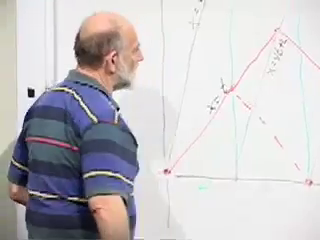
\includegraphics[width=0.72\textwidth]{lecture_01_figure_04.png}\caption{Le rayon lumineux vers l’avant \(x=t\) rencontre la ligne d’univers centrale du référentiel mobile.}\lectureframe{01:02:33}\end{figure}

On peut représenter la géométrie complète sans l’obstruction d’une personne devant le tableau :

\begin{figure}[H]\centering
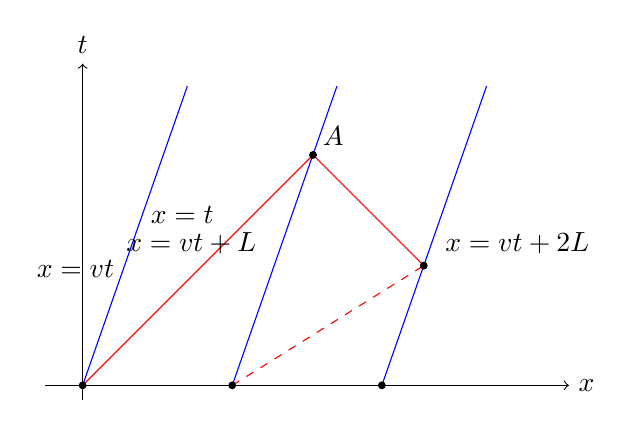
\begin{tikzpicture}[scale=0.95]
\draw[->] (-0.5,0) -- (6.5,0) node[right] {$x$};
\draw[->] (0,-0.2) -- (0,4.3) node[above] {$t$};
\draw[blue] (0,0) -- (1.4,4.0);
\draw[blue] (2.0,0) -- (3.4,4.0);
\draw[blue] (4.0,0) -- (5.4,4.0);
\draw[red] (0,0) -- (3.08,3.08);
\draw[red] (3.08,3.08) -- (4.56,1.60);
\draw[red,dashed] (2.0,0) -- (4.56,1.60);
\fill (0,0) circle (1.5pt);
\fill (2.0,0) circle (1.5pt);
\fill (4.0,0) circle (1.5pt);
\fill (3.08,3.08) circle (1.5pt);
\fill (4.56,1.60) circle (1.5pt);
\node[left] at (0.55,1.55) {$x=vt$};
\node[left] at (2.45,1.9) {$x=vt+L$};
\node[right] at (4.72,1.9) {$x=vt+2L$};
\node[left] at (1.88,2.28) {$x=t$};
\node[above right] at (3.08,3.08) {$A$};
\end{tikzpicture}\caption{Les signaux lumineux déterminent la ligne de simultanéité du référentiel mobile.}\end{figure}

Émettons un rayon lumineux vers la droite depuis l’origine. Notons \(A\) son intersection avec la ligne d’univers centrale. Les deux équations en \(A\) sont
\begin{align}
x&=t,\\
x&=vt+L.
\end{align}
En substituant, on obtient
\begin{equation}
t=vt+L,
\end{equation}
d’où
\begin{equation}
t_A=x_A=\frac{L}{1-v}.
\label{eq:point-a}
\end{equation}

À partir de \(A\), suivons en arrière un rayon lumineux dirigé vers la gauche jusqu’à la ligne d’univers mobile la plus à droite. Son équation est de la forme
\begin{equation}
x+t=b.
\end{equation}
Comme il passe par \(A\), l’équation~\eqref{eq:point-a} détermine la constante :
\begin{equation}
b=x_A+t_A=\frac{2L}{1-v}.
\end{equation}
Le rayon suivi vers l’arrière satisfait donc
\begin{equation}
x+t=\frac{2L}{1-v}.
\label{eq:backward-ray}
\end{equation}

Son intersection avec la ligne d’univers la plus à droite est donnée par
\begin{align}
x+t&=\frac{2L}{1-v},\\
x&=vt+2L.
\end{align}
Éliminons \(x\) :
\begin{align}
(1+v)t
  &=2L\left(\frac{1}{1-v}-1\right)\\
  &=\frac{2Lv}{1-v},
\end{align}
d’où
\begin{equation}
t=\frac{2Lv}{1-v^2}.
\end{equation}
En substituant dans \(x=vt+2L\), on obtient
\begin{equation}
x=\frac{2L}{1-v^2}.
\end{equation}
Les coordonnées elles-mêmes importent moins que leur rapport :
\begin{equation}
\frac{t}{x}=v.
\end{equation}
Ainsi, tout événement simultané avec l’origine selon les horloges mobiles se trouve sur
\begin{equation}
t=vx,
\label{eq:simultaneity-c-one}
\end{equation}
tandis que l’origine mobile suit
\begin{equation}
x=vt.
\label{eq:moving-time-axis}
\end{equation}
Les deux axes sont inclinés symétriquement autour du rayon lumineux à \(45^\circ\).

Tous les points de \(x=vt\) ont la même position primée, \(x'=0\), tandis que leur temps primé varie. Tous les points de \(t=vx\) ont le même temps primé, \(t'=0\), tandis que leur position primée varie. L’une de ces droites est donc l’axe du temps primé et l’autre, l’axe de l’espace primé. Cette longue construction à l’aide de signaux était nécessaire pour déterminer la seconde droite ; on ne pouvait pas la déduire de la seule ligne d’univers mobile.

Pour rétablir les unités usuelles dans l’équation~\eqref{eq:simultaneity-c-one}, il faut écrire
\begin{equation}
t=\frac{v}{c^2}x.
\label{eq:simultaneity-dimensional}
\end{equation}
Le facteur \(c^2\) explique pourquoi la représentation newtonienne fonctionne si bien dans la vie quotidienne. Pour des vitesses très faibles devant \(c\), la pente de la ligne de simultanéité mobile est extrêmement petite.

\begin{figure}[H]\centering
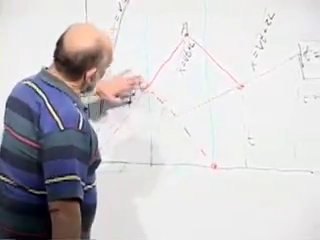
\includegraphics[width=0.72\textwidth]{lecture_01_figure_05.png}\caption{Pour \(c=1\), les axes primés du temps et de la simultanéité sont symétriques par rapport au rayon lumineux.}\lectureframe{01:15:40}\end{figure}

\begin{figure}[H]\centering
\begin{tikzpicture}[scale=1.0]
\draw[->] (-2.2,0) -- (5.2,0) node[right] {$x$};
\draw[->] (0,-0.2) -- (0,4.9) node[above] {$t$};
\draw[red] (0,0) -- (3.9,3.9);
\draw[red] (0,0) -- (-1.8,1.8);
\draw[blue] (0,0) -- (1.8,4.5);
\draw[blue,dashed] (0,0) -- (4.5,1.8);
\node[right] at (3.9,3.9) {$x=t$};
\node[left] at (-1.8,1.8) {$x=-t$};
\node[above] at (1.8,4.5) {$x'=0$};
\node[right] at (4.5,1.8) {$t'=0$};
\end{tikzpicture}\caption{Les axes primés et les rayons lumineux invariants en unités où \(c=1\).}\end{figure}

\section{Dérivation de la transformation de Lorentz}

La géométrie fixe les lieux où chaque coordonnée primée s’annule. Sur l’axe du temps mobile \(x=vt\), il faut que \(x'=0\). Sur l’axe de simultanéité mobile \(t=vx\), il faut que \(t'=0\). Les relations linéaires les plus générales ayant ces ensembles de zéros peuvent s’écrire
\begin{align}
x'&=\frac{x-vt}{F(v)},\\
t'&=\frac{t-vx}{G(v)}.
\label{eq:fg-ansatz}
\end{align}
Les facteurs \(F\) et \(G\) permettent aux échelles des coordonnées primées de différer des échelles galiléennes, bien que les axes aient déjà été localisés. La linéarité découle de l’homogénéité de l’espace et du temps : une translation de l’expérience ne peut modifier la loi de transformation.\editorialnote{Cet argument succinct sur la linéarité explicite une hypothèse utilisée implicitement dans la dérivation au tableau.}

À ce stade, la géométrie nous a appris beaucoup, mais pas tout. Les numérateurs déterminent l’inclinaison des axes. Ils ne déterminent pas l’espacement des unités le long de ces axes. C’est précisément cette information d’échelle restante que représentent \(F(v)\) et \(G(v)\).

Imposons maintenant l’invariance de la vitesse de la lumière. Un rayon dirigé vers la droite, qui satisfait \(x=t\), doit aussi satisfaire \(x'=t'\). Le long de ce rayon,
\begin{align}
x'&=\frac{(1-v)t}{F(v)},\\
t'&=\frac{(1-v)t}{G(v)}.
\end{align}
L’égalité doit tenir en chaque point du rayon, ce qui impose
\begin{equation}
F(v)=G(v).
\end{equation}
Nous pouvons donc écrire
\begin{align}
x'&=\frac{x-vt}{F(v)},\\
t'&=\frac{t-vx}{F(v)}.
\label{eq:common-f}
\end{align}

Cette étape fait intervenir, pour la première fois dans le calcul, une exigence proprement einsteinienne. Une même droite géométrique représente un rayon lumineux pour les deux observateurs ; les deux coordonnées primées doivent donc augmenter à la même vitesse le long de cette droite lorsque \(c=1\). Des facteurs différents dans les deux équations donneraient une vitesse primée différente de l’unité.

Il reste une fonction inconnue. Multiplions l’équation~\eqref{eq:common-f} par \(F(v)\) :
\begin{align}
F(v)x'&=x-vt,\\
F(v)t'&=t-vx.
\end{align}
En multipliant la seconde équation par \(v\), puis en l’ajoutant à la première, on élimine \(t\) et l’on obtient
\begin{equation}
(1-v^2)x=F(v)(x'+vt').
\end{equation}
De même,
\begin{equation}
(1-v^2)t=F(v)(t'+vx').
\end{equation}
La transformation inverse est donc
\begin{align}
x&=\frac{F(v)}{1-v^2}(x'+vt'),\\
t&=\frac{F(v)}{1-v^2}(t'+vx').
\end{align}

Le principe de relativité rend les deux référentiels réciproques. Si la gare voit le train se déplacer à \(+v\), le train voit la gare se déplacer à \(-v\). Les équations inverses doivent donc avoir la même forme que les équations directes, avec le signe de \(v\) inversé. Leurs facteurs de proportionnalité doivent satisfaire
\begin{equation}
\frac{F(v)}{1-v^2}=\frac{1}{F(v)}.
\end{equation}
D’où
\begin{equation}
F(v)^2=1-v^2,
\end{equation}
et la continuité avec la transformation identité pour \(v=0\) sélectionne la racine positive :
\begin{equation}
F(v)=\sqrt{1-v^2}.
\end{equation}

Aucun rayon lumineux particulier n’a servi à ajuster le résultat. Celui-ci découle des axes fixés par la synchronisation, de l’universalité de la vitesse de la lumière et de l’exigence qu’aucun des deux référentiels inertiels ne soit privilégié par rapport à l’autre.

La transformation de Lorentz en unités où \(c=1\) s’écrit
\begin{align}
x'&=\frac{x-vt}{\sqrt{1-v^2}},\\
t'&=\frac{t-vx}{\sqrt{1-v^2}}.
\label{eq:lorentz-c-one}
\end{align}
Sa transformation inverse est
\begin{align}
x&=\frac{x'+vt'}{\sqrt{1-v^2}},\\
t&=\frac{t'+vx'}{\sqrt{1-v^2}}.
\end{align}

\begin{figure}[H]\centering
\includegraphics[width=0.76\textwidth]{lecture_01_figure_06.png}\caption{La transformation de Lorentz complète en unités où \(c=1\), écrite au tableau.}\lectureframe{01:32:38}\end{figure}

La nouveauté essentielle apparaît déjà dans l’équation du temps. Le temps n’est pas simplement transmis sans changement d’un référentiel à l’autre. La coordonnée temporelle primée combine le temps et la position non primés. Par conséquent, \(t=\text{constant}\) et \(t'=\text{constant}\) décrivent des ensembles différents d’événements.

Le terme de mélange n’est pas une correction facultative ajoutée après coup. Sans lui, la droite \(t'=0\) resterait horizontale, la simultanéité à distance demeurerait universelle et la transformation ne pourrait pas préserver la vitesse de la lumière.

\section{Rétablir la vitesse de la lumière et vérifier le résultat}

Lorsque \(c\ne1\), la cohérence dimensionnelle rétablit les facteurs manquants. Le rapport \(v^2/c^2\) est sans dimension, tandis que \((v/c^2)x\) a les dimensions d’un temps. On a donc
\begin{align}
x'&=\frac{x-vt}{\sqrt{1-v^2/c^2}},\\
t'&=\frac{t-(v/c^2)x}{\sqrt{1-v^2/c^2}}.
\label{eq:lorentz-dimensional}
\end{align}
On obtient la transformation inverse en inversant le signe de \(v\) :
\begin{align}
x&=\frac{x'+vt'}{\sqrt{1-v^2/c^2}},\\
t&=\frac{t'+(v/c^2)x'}{\sqrt{1-v^2/c^2}}.
\end{align}
En introduisant
\begin{equation}
\gamma=\frac{1}{\sqrt{1-v^2/c^2}}
\end{equation}
on obtiendrait la forme compacte usuelle, mais l’écriture avec le dénominateur permet de suivre la dérivation.

Numériquement, \(c\simeq3\times10^8\,\mathrm{m/s}\), donc \(c^2\simeq9\times10^{16}\,\mathrm{m^2/s^2}\). Le grand dénominateur rend imperceptibles, dans la plupart des expériences mécaniques, l’inclinaison de la simultanéité et le facteur \(v^2/c^2\). Leur petitesse explique le succès de Galilée ; elle ne rétablit pas le temps absolu.

\begin{figure}[H]\centering
\includegraphics[width=0.76\textwidth]{lecture_01_figure_07.png}\caption{La transformation de Lorentz après rétablissement des facteurs de \(c\).}\lectureframe{01:35:58}\end{figure}

Deux vérifications s’imposent immédiatement. Commençons par \(v\ll c\). Alors, \(v^2/c^2\) est négligeable et, pour des distances ordinaires, le terme de relativité de la simultanéité \(vx/c^2\) l’est aussi. L’équation~\eqref{eq:lorentz-dimensional} se réduit à
\begin{equation}
t'\approx t,\qquad x'\approx x-vt.
\end{equation}
On retrouve la relativité galiléenne comme approximation aux faibles vitesses.

Deuxièmement, considérons un rayon lumineux. Une fois \(c\) rétabli, un rayon se propageant vers la droite obéit à \(x=ct\), et non à \(x=t\). La substitution donne
\begin{align}
x'&=\frac{(c-v)t}{\sqrt{1-v^2/c^2}},\\
t'&=\frac{(1-v/c)t}{\sqrt{1-v^2/c^2}}.
\end{align}
Puisque \(c-v=c(1-v/c)\),
\begin{equation}
x'=ct'.
\end{equation}
L’observateur primé mesure la même vitesse \(c\). Pour un rayon se propageant vers la gauche, la substitution de \(x=-ct\) donne de même
\begin{equation}
x'=-ct'.
\end{equation}
La transformation décrit correctement la lumière se propageant dans les deux directions.

La distinction entre \(x=t\) et \(x=ct\) constitue une vérification dimensionnelle instructive. La première expression n’est correcte que dans un système d’unités où \(c=1\). Rétablir les unités usuelles dans la transformation tout en laissant l’équation du rayon en unités naturelles reviendrait à mélanger deux conventions et conduirait à un résultat erroné. La cohérence dimensionnelle permet de repérer immédiatement l’erreur.

\section{Le critère du point milieu}

\begin{classroomqa}
\audiencequestion{Un observateur reçoit deux éclairs lumineux au même instant, mais il ne se trouve pas à mi-distance de leurs sources. Peut-il en conclure que les éclairs ont été émis simultanément ?
\lecturetimestamp{01:42:55}}
\lecturerresponse{Non. Des temps d’arrivée égaux impliquent des temps d’émission égaux uniquement pour l’observateur situé à mi-distance spatiale des deux sources dans le référentiel considéré. Un récepteur plus proche de l’une des sources peut recevoir les deux éclairs en même temps alors que l’éclair le plus éloigné a été émis plus tôt. Dans la construction en mouvement, la ligne d’univers du point milieu \(x=vt+L\) est donc essentielle. On suit le rayon lumineux dirigé vers l’avant \(x=t\) jusqu’à ce qu’il rencontre ce point milieu, puis on trace un rayon lumineux vers l’arrière jusqu’à \(x=vt+2L\). Cet événement à la seconde extrémité, et non un événement quelconque d’arrivée simultanée ailleurs, est simultané à l’origine selon le référentiel en mouvement.}
\end{classroomqa}

Nous sommes parvenus à la transformation complète des coordonnées, mais pas encore à ses conséquences les plus connues. Nous examinerons ensuite la contraction des longueurs, la dilatation du temps et le temps propre, puis la quantité de mouvement et l’énergie relativistes. Les bases sont déjà posées : chaque référentiel inertiel ne peut appliquer les mêmes lois et mesurer la même vitesse de la lumière que parce que l’espace et le temps se mélangent, et parce que la simultanéité à distance est propre à un référentiel, et non au monde en soi.
